\chapter{Conclusions}

In this chapter the final results of this master thesis are presented.

The results of a forecast of atmospheric effects for the LSPE/Strip
instrument is presented first. Then, future prospects following this work
are given.

\section{A Forecast for the LSPE/Strip Instrument}

Using the methods discussed in \autoref{ch:comparison_quijote}, we have
produced a forecast of the seasonal variations of atmospheric
brightness temperature for the Q-band of the Strip instrument of the LSPE
experiment, at \SI{43}{\giga\hertz}. The Strip telescope is briefly
Described in \autoref{ch:lspe_strip}.

We have calculated a population of atmospheric brightness temperatures for each
hour of the typical day of each month of the year, using CAL. As usual, the
\texttt{Weather} class has been initialized with the CDF \texttt{.fits}
file for Pico del Teide. Every statistical population contains exactly
\num{9900} elements. The expectation values of each population and the
corresponding standard errors has been obtained, using median as estimator.
As before, standard errors have been computed splitting the statistical
populations in \num{10} samples of the same number of elements and
applying a bootstrapping technique.

\autoref{fig:tatm_cal} shows the annual variations of
$T_\text{atm}\qty(\SI{43}{\giga\hertz})$ and the corresponding standard
errors. Instead, \autoref{fig:median_tatm_matrix_cal} represents the same
data in a color map. Several pieces of information can be extracted from
these graphs.

\begin{figure}
        \centering
        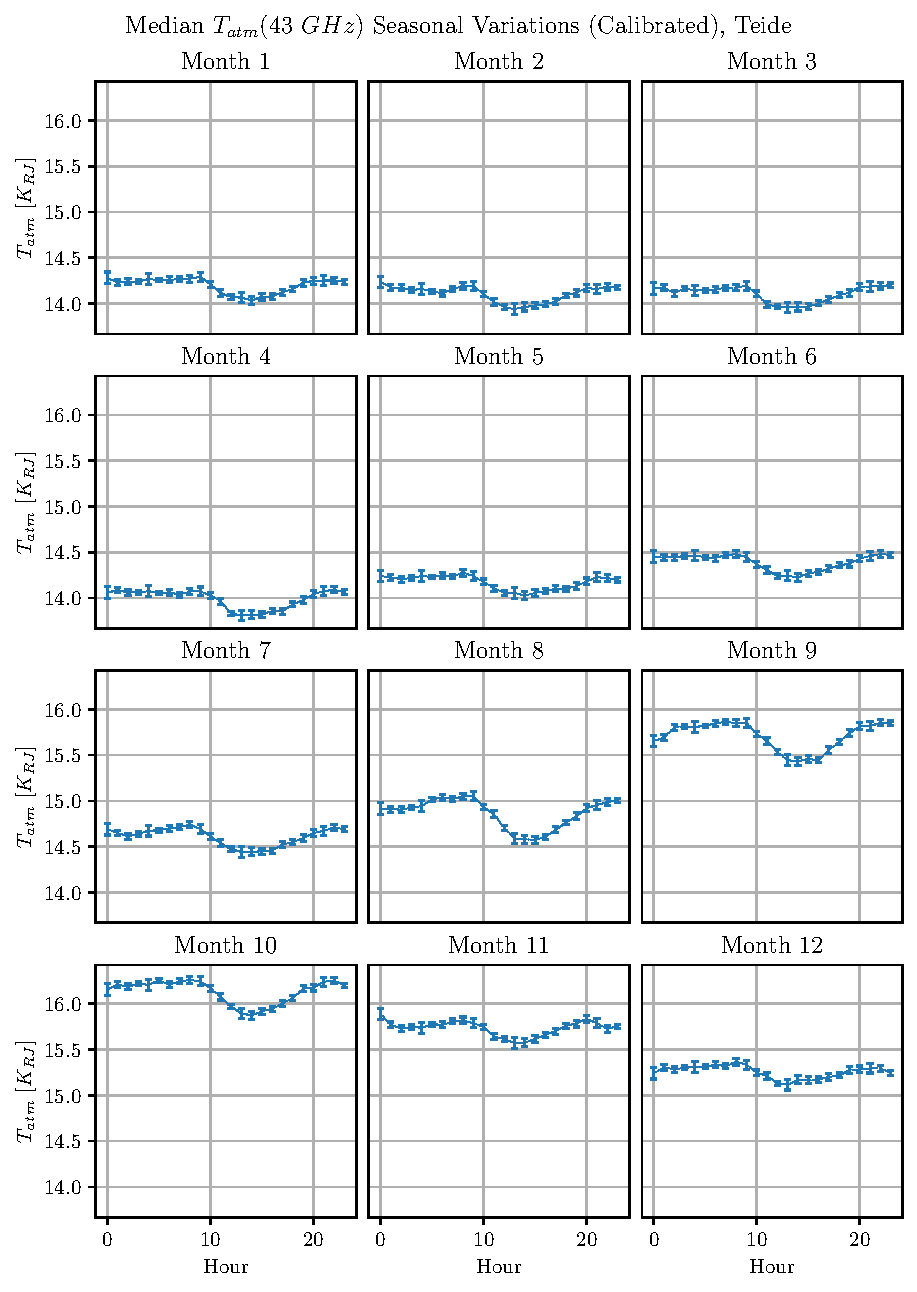
\includegraphics[width=0.96\textwidth]{TATM_cal}
        \caption{Median seasonal variations of atmospheric brightness
        temperature at \SI{43}{\giga\hertz} for Pico del Teide. Error bars
        have been tripled in size to make them more visible.}
        \label{fig:tatm_cal}
\end{figure}

\begin{figure}
        \centering
        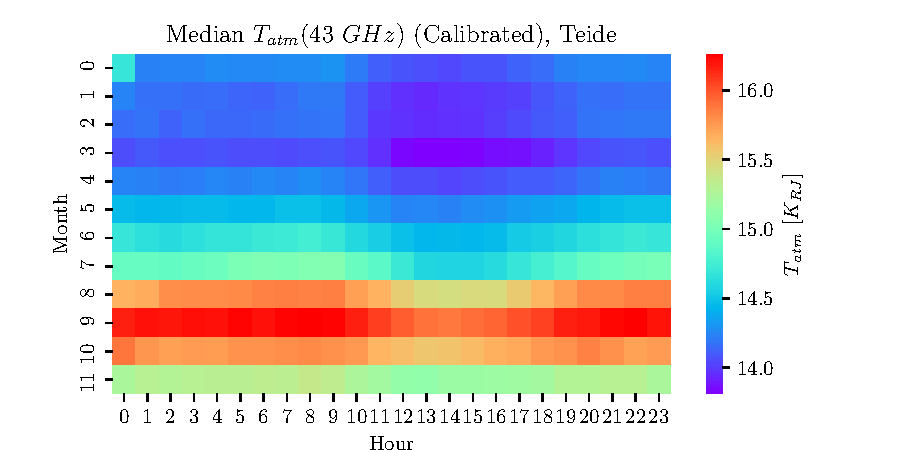
\includegraphics[width=\textwidth]{Median_TATM_Matrix_cal}
        \caption{Seasonal matrix for median atmospheric brightness
        temperature at \SI{43}{\giga\hertz} for Pico del Teide.}
        \label{fig:median_tatm_matrix_cal}
\end{figure}

\autoref{tab:mean_tatm_month} contains average atmospheric brightness
temperatures at \SI{43}{\giga\hertz} and the corresponding errors for each
month of the year. We have obtained these values averaging the data of each
month over the hours of the day. As we can see, the extra loading of the
atmosphere on the detectors is maximum in October and in general assumes
values over $3\sigma$ above its annual average of \SI{14.77 \pm
0.21}{\kelvin} in September, October and November. In fact, these months
are characterized by great values of PWV, as we can learn from
\autoref{fig:teide_seasonal_matrices_vertical}.

\begin{table}
        \renewcommand{\arraystretch}{1.5}
        \centering
        \begin{tabular}{p{5cm} r}
                \hline
                Month & Average $T_\text{atm}\qty(\SI{43}{\giga\hertz})\
                \qty[\si{\kelvin}]$ \\
                \hline
                \hline
                Gen \dotfill & \num{14.198 \pm 0.017} \\
                Feb \dotfill & \num{14.106 \pm 0.018} \\
                Mar \dotfill & \num{14.107 \pm 0.017} \\
                Apr \dotfill & \num{13.991 \pm 0.021} \\
                May \dotfill & \num{14.169 \pm 0.016} \\
                Jun \dotfill & \num{14.390 \pm 0.018} \\
                Jul \dotfill & \num{14.608 \pm 0.020} \\
                Aug \dotfill & \num{14.865 \pm 0.032} \\
                Sep \dotfill & \num{15.707 \pm 0.031} \\
                Oct \dotfill & \num{16.131 \pm 0.026} \\
                Nov \dotfill & \num{15.733 \pm 0.017} \\
                Dec \dotfill & \num{15.256 \pm 0.014} \\
                \noalign{\smallskip}
                \hline
        \end{tabular}
        \caption{Monthly average atmospheric brightness temperature at
        \SI{43}{\giga\hertz} for Pico del Teide.}
        \label{tab:mean_tatm_month}
\end{table}

\autoref{tab:mean_tatm_dayly_esc} displays average daily excursion of
atmospheric brightness temperature for each month of the year. We have used
an analogous approach to that described above for average $T_\text{atm}$ to
obtain these values. The daily excursion is maximum in August and in
general it takes values over $3\sigma$ above its annual average of
\SI{0.312 \pm 0.023}{\kelvin} in the months of August, September and
October. Again, from \autoref{fig:teide_seasonal_matrices_vertical} we
learn that these are the months of the year in which surface pressure
takes its greatest values.

\begin{table}
        \renewcommand{\arraystretch}{1.5}
        \centering
        \begin{tabular}{p{5cm} r}
                \hline
                Month & Average $\Delta
                T_\text{atm}\qty(\SI{43}{\giga\hertz})$
                Day [\si{\kelvin}] \\
                \hline
                \hline
                Gen \dotfill & \num{0.258 \pm 0.022} \\
                Feb \dotfill & \num{0.296 \pm 0.015} \\
                Mar \dotfill & \num{0.240 \pm 0.017} \\
                Apr \dotfill & \num{0.284 \pm 0.016} \\
                May \dotfill & \num{0.250 \pm 0.013} \\
                Jun \dotfill & \num{0.253 \pm 0.017} \\
                Jul \dotfill & \num{0.301 \pm 0.022} \\
                Aug \dotfill & \num{0.479 \pm 0.023} \\
                Sep \dotfill & \num{0.434 \pm 0.022} \\
                Oct \dotfill & \num{0.387 \pm 0.033} \\
                Nov \dotfill & \num{0.314 \pm 0.030} \\
                Dec \dotfill & \num{0.251 \pm 0.014} \\
                \noalign{\smallskip}
                \hline
        \end{tabular}
        \caption{Average daily excursion of atmospheric brightness
        temperature for Pico del Teide at \SI{43}{\giga\hertz} for each
        month.}
        \label{tab:mean_tatm_dayly_esc}
\end{table}

Instead, the average annual excursion of atmospheric brightness temperature
can be obtained from \autoref{tab:mean_tatm_month}. It takes a value of
\SI{2.139 \pm 0.033}{\kelvin}, showing that the extra load on detectors
from atmospheric effects is subjected to relatively small daily variations
as compared to overall annual variations.

The findings presented in this section can be used as a starting point to
forecast the maximum sensitivity that Strip radiometers can reach due to
atmospheric effects.  We show some preliminaries results in
\autoref{sensitivity}.

\section{Future Prospects}
